\documentclass[11pt,a4j]{jarticle}
\usepackage[dvipdfmx]{graphicx,color}
\usepackage{wrapfig}
\usepackage{amssymb}
\setlength{\topmargin}{-1.5cm}
\setlength{\textwidth}{15.5cm}
\setlength{\textheight}{25.2cm}
\newlength{\minitwocolumn}
\setlength{\minitwocolumn}{0.5\textwidth}
\addtolength{\minitwocolumn}{-\columnsep}
%\addtolength{\baselineskip}{-0.1\baselineskip}
%
\def\Mmaru#1{{\ooalign{\hfil#1\/\hfil\crcr
\raise.167ex\hbox{\mathhexbox 20D}}}}
%
\begin{document}
\newcommand{\fat}[1]{\mbox{\boldmath $#1$}}
\newcommand{\D}{\partial}
\newcommand{\w}{\omega}
\newcommand{\ga}{\alpha}
\newcommand{\gb}{\beta}
\newcommand{\gx}{\xi}
\newcommand{\gz}{\zeta}
\newcommand{\vhat}[1]{\hat{\fat{#1}}}
\newcommand{\spc}{\vspace{0.7\baselineskip}}
\newcommand{\halfspc}{\vspace{0.3\baselineskip}}
\bibliographystyle{unsrt}
%\pagestyle{empty}
\newcommand{\twofig}[2]
 {
   \begin{figure}[h]
     \begin{minipage}[t]{\minitwocolumn}
         \begin{center}   #1
         \end{center}
     \end{minipage}
         \hspace{\columnsep}
     \begin{minipage}[t]{\minitwocolumn}
         \begin{center} #2
         \end{center}
     \end{minipage}
   \end{figure}
 }
%%%%%%%%%%%%%%%%%%%%%%%%%%%%%%%%%
%\vspace*{\baselineskip}
\vspace{2mm}
\begin{center}
{\LARGE \bf 
粗視化分子動力学法による\\水和モンモリロナイトの組織構造シミュレーション\\
} 
 ○木本 和志$^1$、河村 雄行$^2$、牧野 仁史$^3$\\
1岡山大学環境生命科学研究科(〒700-8530岡山市北区津島中3-1-1)\\
2東京工業大学工学院(〒152-8550目黒区大岡山2-12-1)\\
3日本原子力研究開発機構核燃料サイクル工学研究所\\
(〒319-1112 茨城県那珂郡東海村村松4-33)
\end{center}
%%%%%%%%%%%%%%%%%%%%%%%%%%%%%%%%%%%%%%%%%%%%%%%%%%%%%%%%%%%%%%%%
\section{緒言}
モンモリロナイトはSiO4四面体とAl(OH)6八面体が2:1で積層した層状ケイ酸塩鉱物の一種で、分子同士が陽イオンを介在して積層構造を作ることが知られている。積層した分子の層間には、陽イオンに水和する形で水分が取り込まれるため、吸湿によってモンモリロナイトは膨潤する。モンモリロナイトの透水性や物質拡散特性といった工学的に重要なマクロ物性を評価するためには、湿潤環境下で、分子がどのように積層し含水した多孔質構造を作るかを調べることが重要である。しかしながら、モンモリロナイト分子は、厚さが約1nm,幅が最大で1μm程度の微細かつ扁平な分子で、水分分布や積層構造、すなわち組織構造を顕微鏡等で直接観察することができない。本稿では、モンモリロナイトの組織構造を計算科学的な方法で調べることを目的として、粗視化分子動力学法によって行った粘土含水系の圧縮凝集に関する2次元シミュレーションの結果を報告する。
\section{方法}
\begin{wrapfigure}[11]{r}[0mm]{60mm}
	\centering
	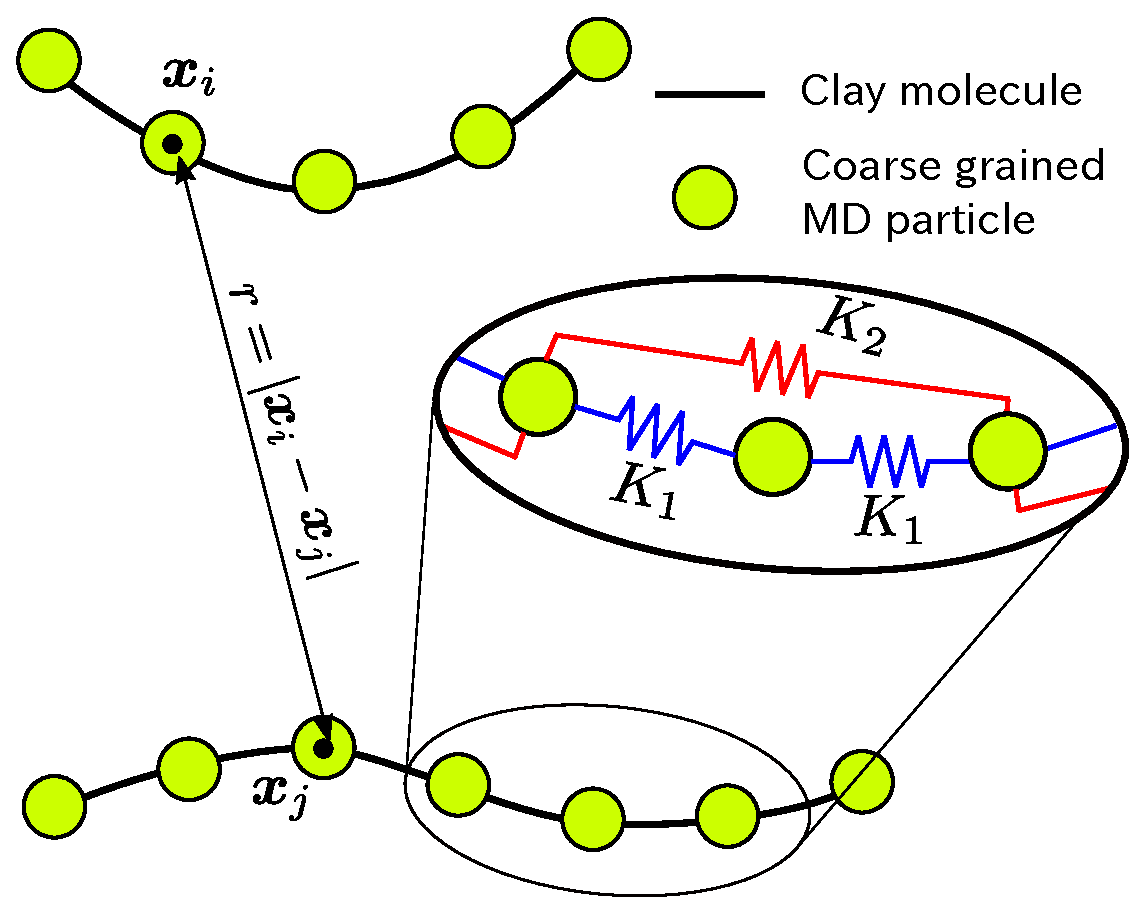
\includegraphics[keepaspectratio,width=50mm]{Figs/cg_model.eps}
	\caption{モンモリロナイト分子の粗視化MDモデル}
	\label{fig:fig1}
\end{wrapfigure}
モンモリロナイトの分子構造や水和挙動は、これまで、分子動力学法(MD)を用いて詳しく調べられ、ナノメートルスケールでの物性は次第に明らかになってきている[1]。一方、組織構造のシミュレーションは、多数の分子からなる系を扱う必要があることから、全原子MDでの解析は、計算負荷が高く困難である。そこでここでは、モンモリロナイト分子の単位構造と水和水を一つの粒子に粗視化したMD計算を行う。粗視化MDでは、一つのモンモリロナイト分子を、粗視化粒子を1次元的につないだビーズモデルで表現する(図1)。同一分子内の粒子間と、異なる分子に属する粒子間には相互作用力を定義し、粗視化粒子系の運動方程式を解くことで、分子の変形と運動を解析する。その際、分子内での粒子間力は、分子の伸縮と屈曲に関する剛性を付与する2種類の線形バネで、図1のように与える。一方、分子間の粒子間力はレナードジョーンズ(LJ)ポテンシャル:
で与える。これらのこれら相互作用力のパラメータは、別途行った全原子MD計算の結果を踏まえ、以下のように設定した。
なお、LJポテンシャルの基準距離σは、分子間の接近限界を定めるため、σの大小で水和水の量を
表現する。ただし、各粗視化粒子が持つ水和水量は、次のようにして計算途上で更新する。はじめに、指定された粗視化粒子に対して、別の粒子をランダムに一つ選ぶ。これらの粒子間で水分の授受が発生したと仮定し、その結果生ずるポテンシャルエネルギーの増減を計算する。エネルギーが下がる場合のみ、水分の授受が発生するとして各々の粒子のσ値を実際に変更する。これを一定の計算ステップ間隔で全ての粒子について行うことで、系全体がよりエネルギーの低い状態に向かうようにして計算を進める。
\begin{equation}
	U(\fat{x}_i,\fat{x}_j)=4\varepsilon
	\left\{ \left(\frac{\sigma}{r}\right)^{12}-
	\left( \frac{\sigma}{r}\right)^6\right\}, 
	\ \ \left(r=\left| \fat{x}_i-\fat{x}_j\right|\right)\hspace{10mm}
\end{equation}
\begin{equation}
	K  = 2,000[{\rm N / m}],   K  = 4000[{\rm N / m}],  \varepsilon = 1.0\times10     [{\rm Nm}]
\end{equation}
\section{結果}
%--------------------
\begin{figure}[h]
	\begin{center}
	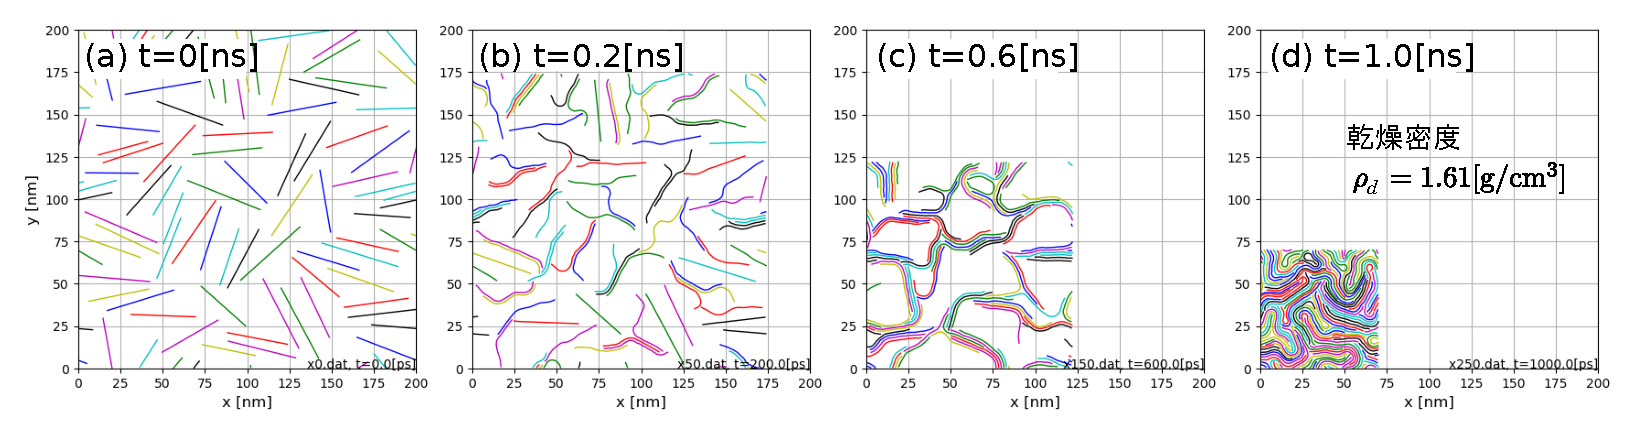
\includegraphics[width=1.0\linewidth]{Figs/revs.eps} 
	\end{center}
	\caption{水和モンモリロナイトの圧縮凝集シミュレーションの結果} 
	\label{fig:fig2}
\end{figure}
%--------------------
\begin{wrapfigure}[14]{r}[0mm]{80mm}
	\centering
	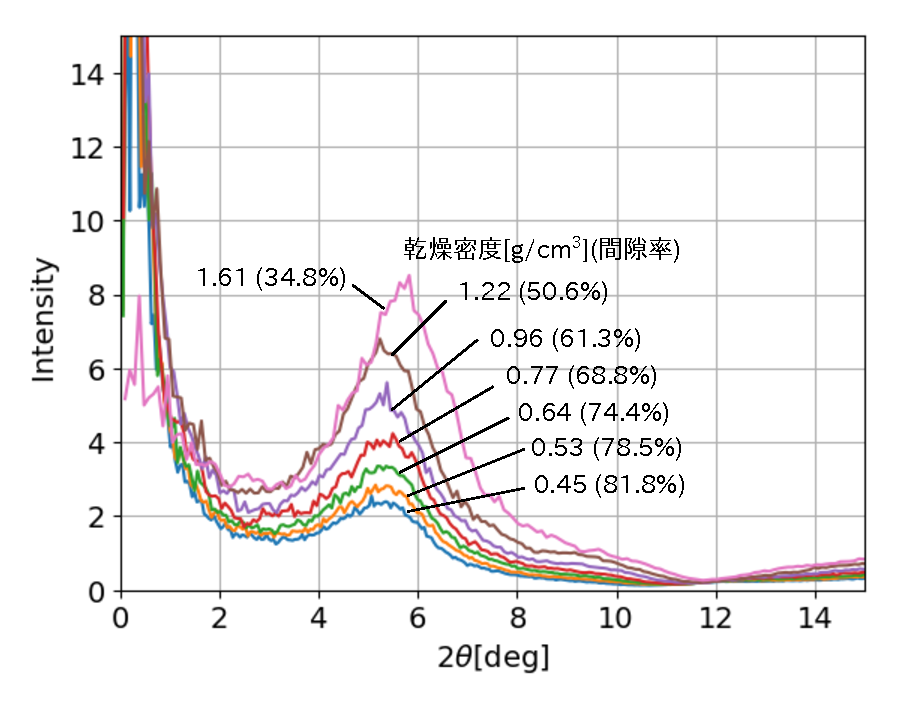
\includegraphics[keepaspectratio,width=75mm]{Figs/xrd.eps}
	\caption{粗視化MD計算の結果から合成したX線回折パターン}
	\label{fig:fig3}
\end{wrapfigure}
図2に、計算結果の一例を示す。この図は、長さの異なる80の分子を含む周期構造を考え、そのユニットセルを一定の速度で各辺を60$\%$
圧縮したときの結果で、t=0[ns]が初期状態を、t=1[ns]が圧縮終了時のユニットセル内の分子配置を示している。分子を構成する粗視化粒子の総数は3,194個で、分子の長さは平均が40[nm]、標準偏差が10[nm]の正規分布でランダムに与えている。水分量は二層膨潤状態に相当するよう、初期状態ではすべての粗視化粒子でσ=1.5[nm]した。ユニットセルの圧縮に伴い、当初、均一に分散した直線状の分子が、次第に屈曲しながら分子間力によって積層する様子が見られる。また、t=0.6[ns]の時点では、積層した分子間に大きな空隙ができるが、さらに圧縮を進めるとそれらの空隙も消失し、非常に密に充填された組織構造が得らえる。最終的に得られた組織構造では、屈曲して積層した分子同士が互いに絡み合うように配置され、基準となる積層構造単位や規則性を見出すことは難しい。
次に、圧縮凝集シミュレーションの結果から計算したX線回折パターンを図3に示す。このグラフは、圧縮終了までの7つの時間ステップで得られた分子配置に対し、電荷密度分布の波数スペクトルを計算することで合成したX線回折パターンである。簡単のため、電荷密度は分子内で一様に分布すると仮定している。横軸は回折角度を、縦軸はX線強度を示し、圧縮の進行にともない5~6度方向のピークが次第に際立ってくる様子が見られる。また、5度付近の回折ピークは、比較的密度の低い段階から見られ、ピーク方向はあまり大きく変わらない。これは、圧縮の早い時点で積層構造が形成されあとは、分子間隔が密になっても、互いに積層する分子の数が大きく変化しないことを意味している。なお、計算を行った系が小さいことから、X線回折パターンはあまり滑らかになっていないが、ピーク角度は、二層膨潤状態にある粘土のX線回折ピークと概ね一致しており、本シミュレーションの妥当性を一部裏付ける結果が得られている。
\section{まとめ}
本稿では、粗視化MDによって計算した水和モンモリロナイトの組織構造とそのX線回折パターンを示し、X線回折ピークは概ね実験で得られる結果に一致することを述べた。今後は、より大きな系で同様な計算を行い、実験で得たX線回折パターンと比較すること、3次元系でのシミュレーションを行うことが課題となる。
参考文献
\begin{thebibliography}{99}
\bibitem{Warren}
	B.E. Warren, "X-ray diffraction", Dover Publication, New York, 1990.
\bibitem{Koide}
	小出昭一郎,"物理現象のフーリエ解析", ちくま学芸文庫, 2018.
\end{thebibliography}

\end{document}
%%%%%%%%%%%%%%%%%%%%%%%%%%%%%%%%%%%%%%%%%%%%%%%%%%%%%%

